\chapter{Manual de Utilização da Bancada}

O primeiro contato do usuário é com a tela inicial. Para dar início ao teste ele deverá clicar em \textbf{Inicial Teste} que está localizado no menu lateral a esquerda. O usuário terá a opção de escolher entre três testes, sendo eles: teste por velocidade fixa, teste por velocidade variável e teste por temperatura. Os tipos de teste estão ilustrados na Figura \ref{img:testes}.

\begin{figure}[h]
	\centering
	\label{img:testes}
		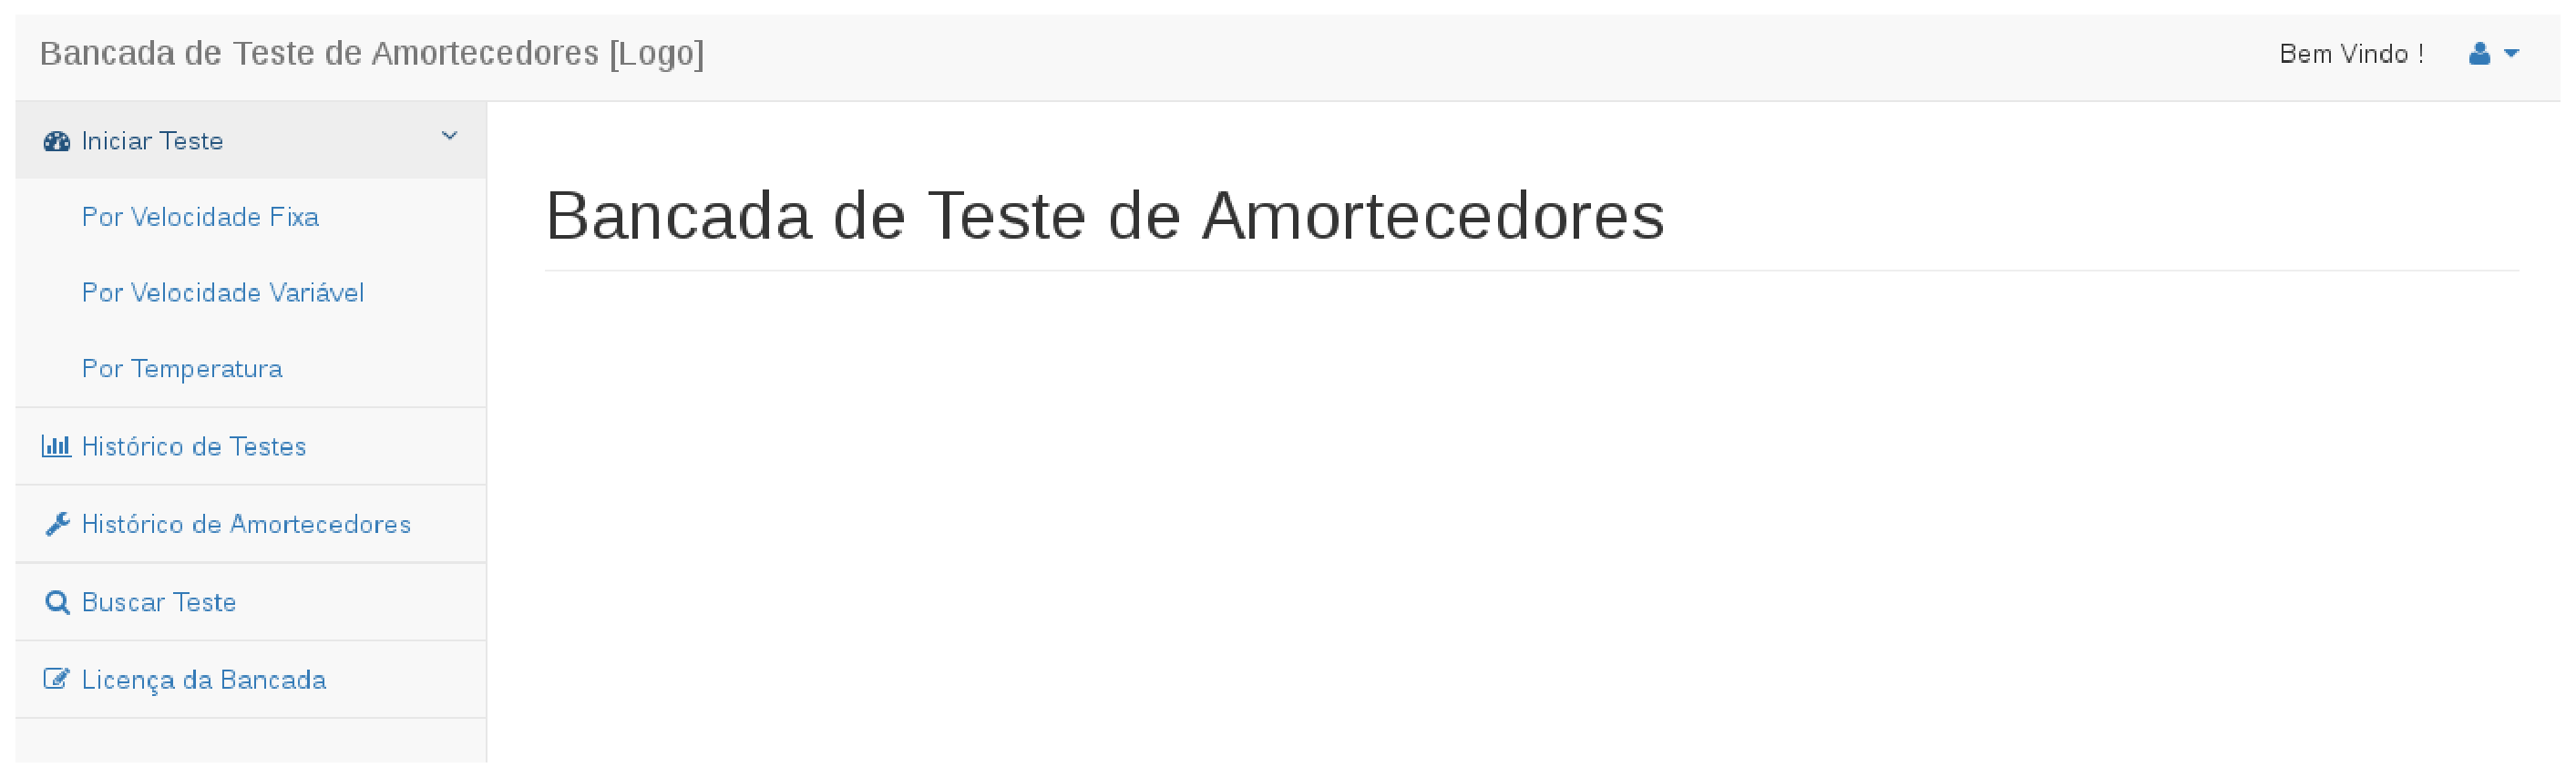
\includegraphics[width=1\textwidth]{figuras/testes.eps}
	\caption{Testes realizados pelo sistema}
\end{figure}

\section{Teste por velocidade fixa}

Para a realização de um teste o usuário deverá estar \textit{logado} no sistema. No momento em que ele clicar no link \textbf{Iniciar Teste -> Por velocidade fixa}, localizado no menu lateral esquerdo, ele será redirecionado para tela de login, Figura \ref{img:login},caso ainda não esteja logado no sistema, ou irá para a página do teste. 

\begin{figure}[h]
	\centering
	\label{img:login}
		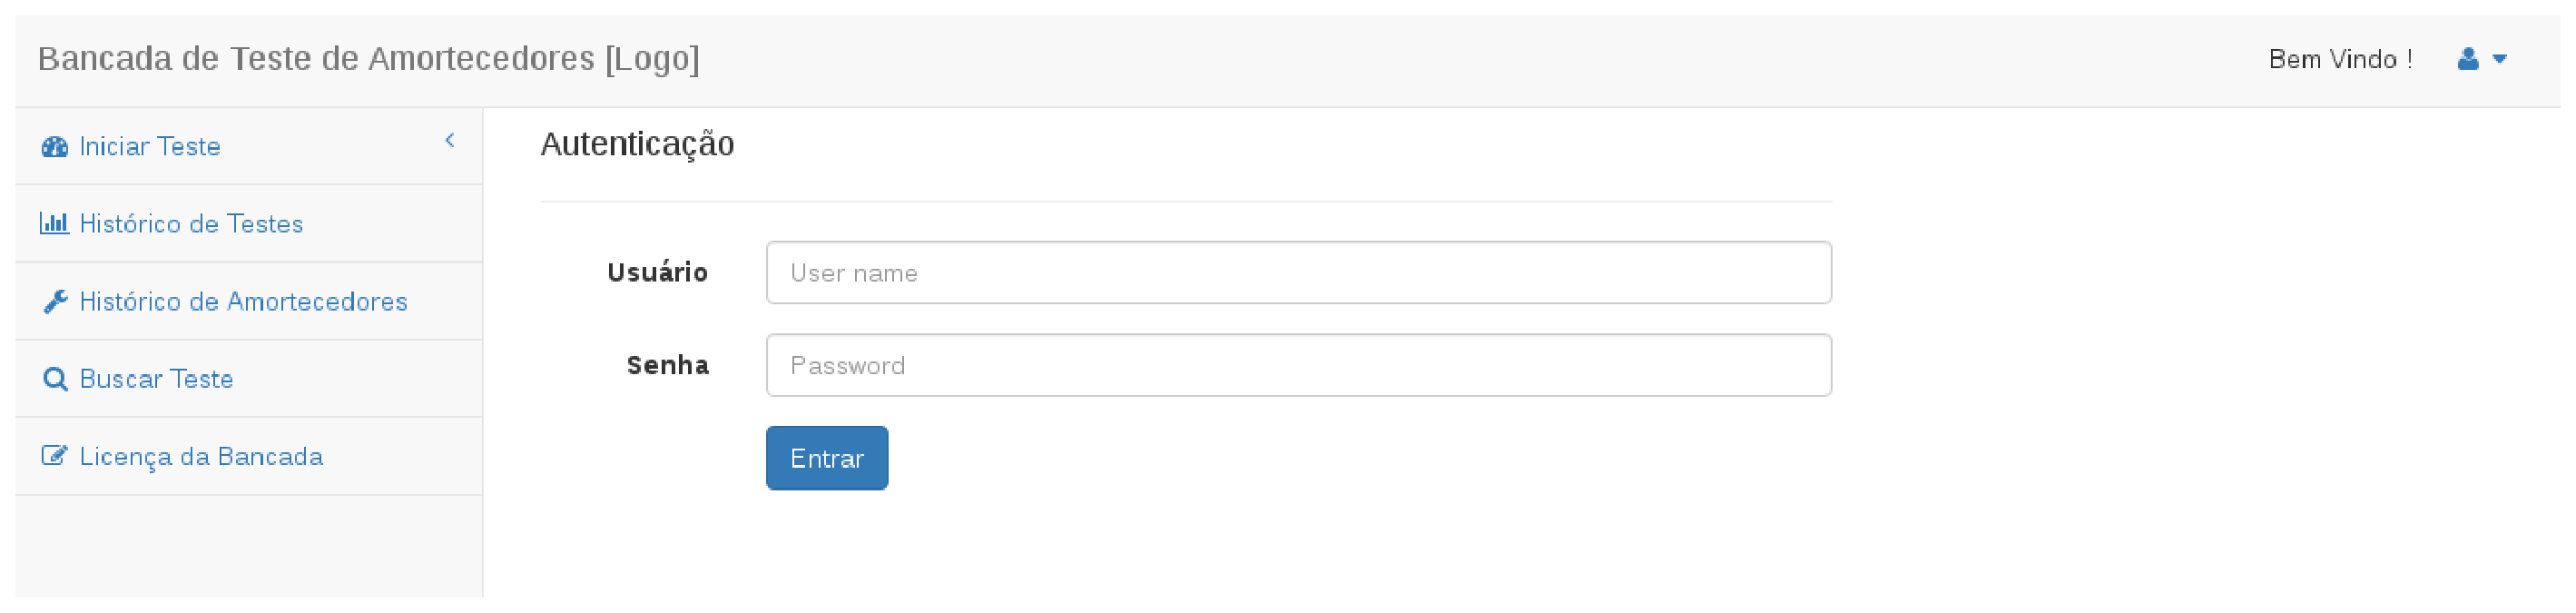
\includegraphics[width=1\textwidth]{figuras/login.eps}
	\caption{Tela de autenticação}
\end{figure}


Na página \textbf{teste por velocidade fixa} terá uma seção referente aos dados do amortecedor e outra seção para informar os dados do teste. Na seção que contém os dados do amortecedor, ao digitar o código de um amortecedor, caso ele já esteja cadastrado no sistema, seus dados serão recuperados e preenchidos automaticamente. Quando o usuário insere o código de um amortecedor que ainda não foi cadastrado e insere seus dados, este será cadastrado no sistema de forma automática. A Figura \ref{img:teste_fixo_um} apresenta os campos necessários para realizar o cadastro do amortecedor.

\begin{figure}[h]
	\centering
	\label{img:teste_fixo_um}
		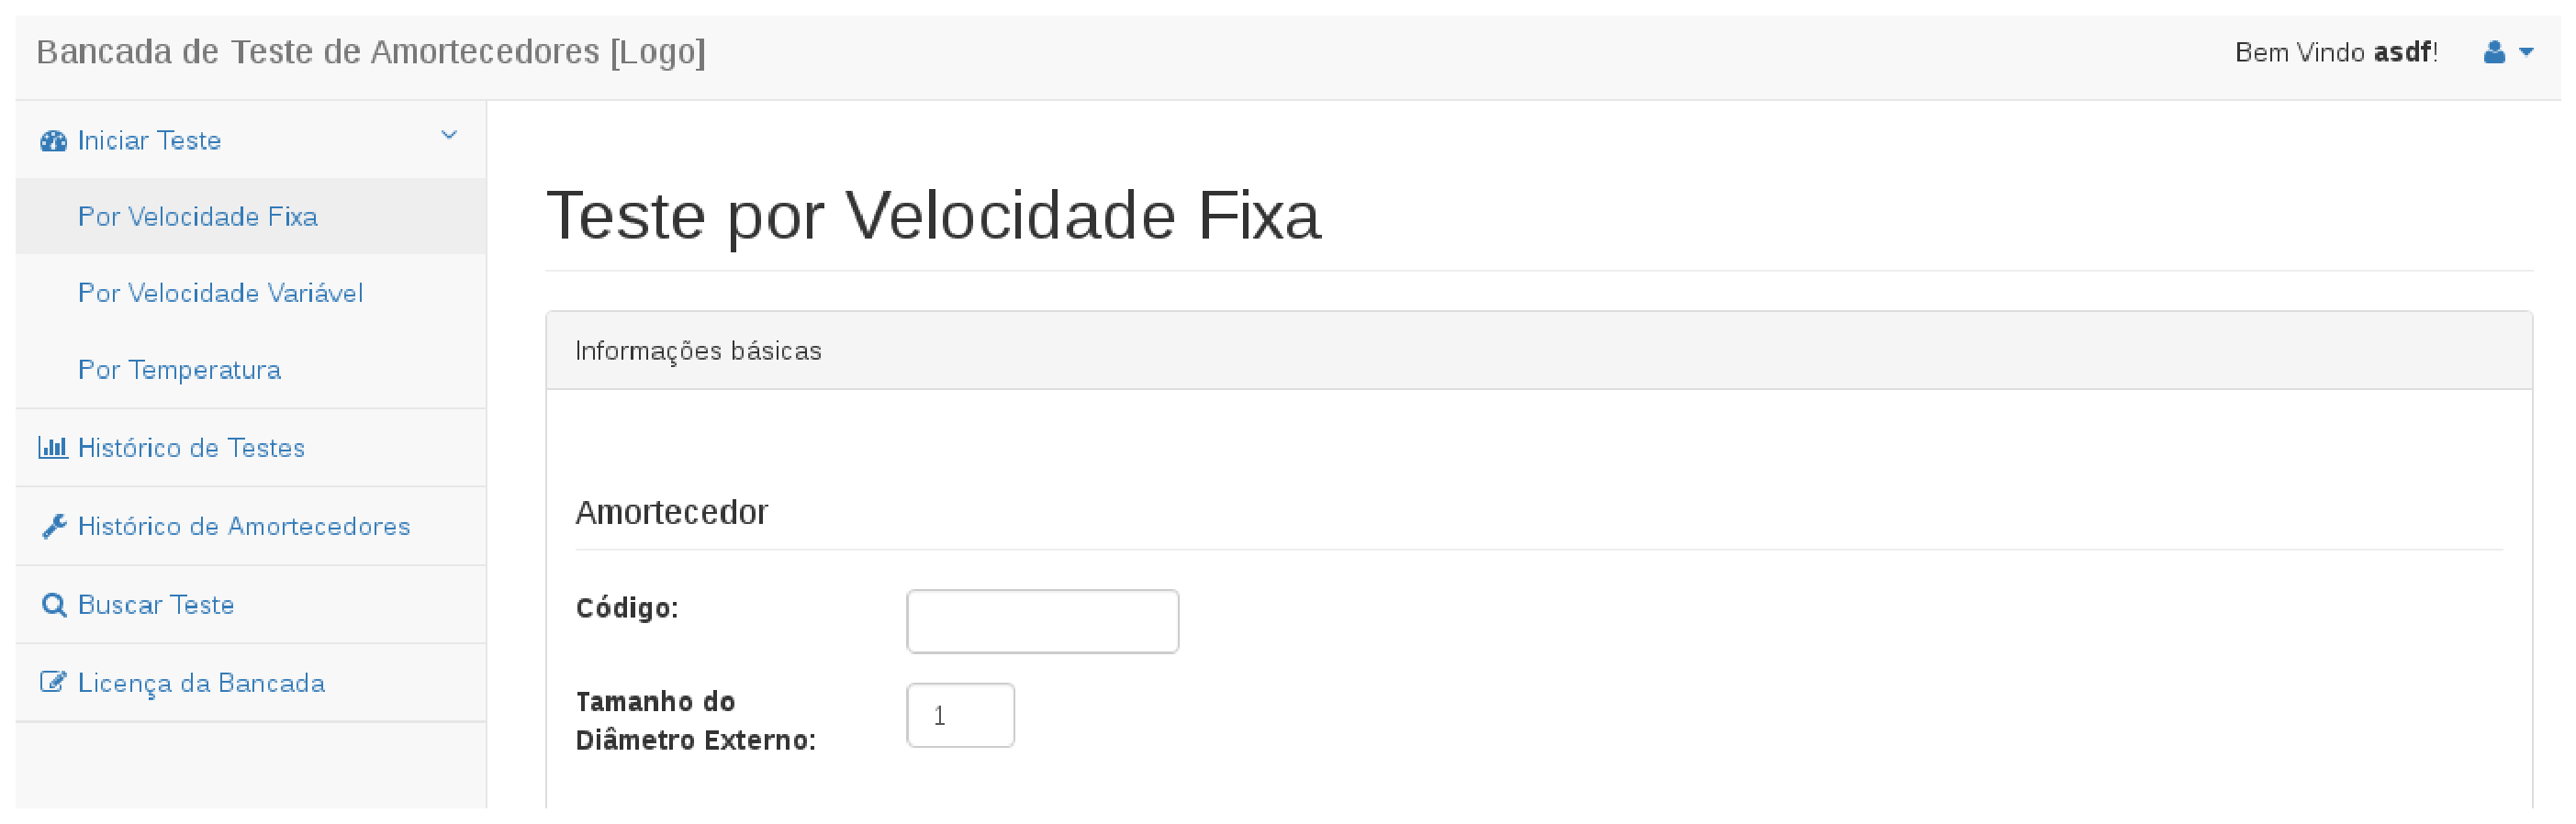
\includegraphics[width=1\textwidth]{figuras/dados_amortecedor.eps}
	\caption{Campos do amortecedor}
\end{figure}

Os dados referentes ao amortecedor são armazenados apenas com o intuito de facilitar a inserção dos dados, eles não influenciam no resultado do teste. O usuário irá inserir o \textit{código} do amortecedor e o \textit{diâmetro externo}. 

A Figura \ref{img:teste_fixo_dois} apresenta o restante da página contendo os campos referentes ao teste. 

\begin{figure}[h]
	\centering
	\label{img:teste_fixo_dois}
		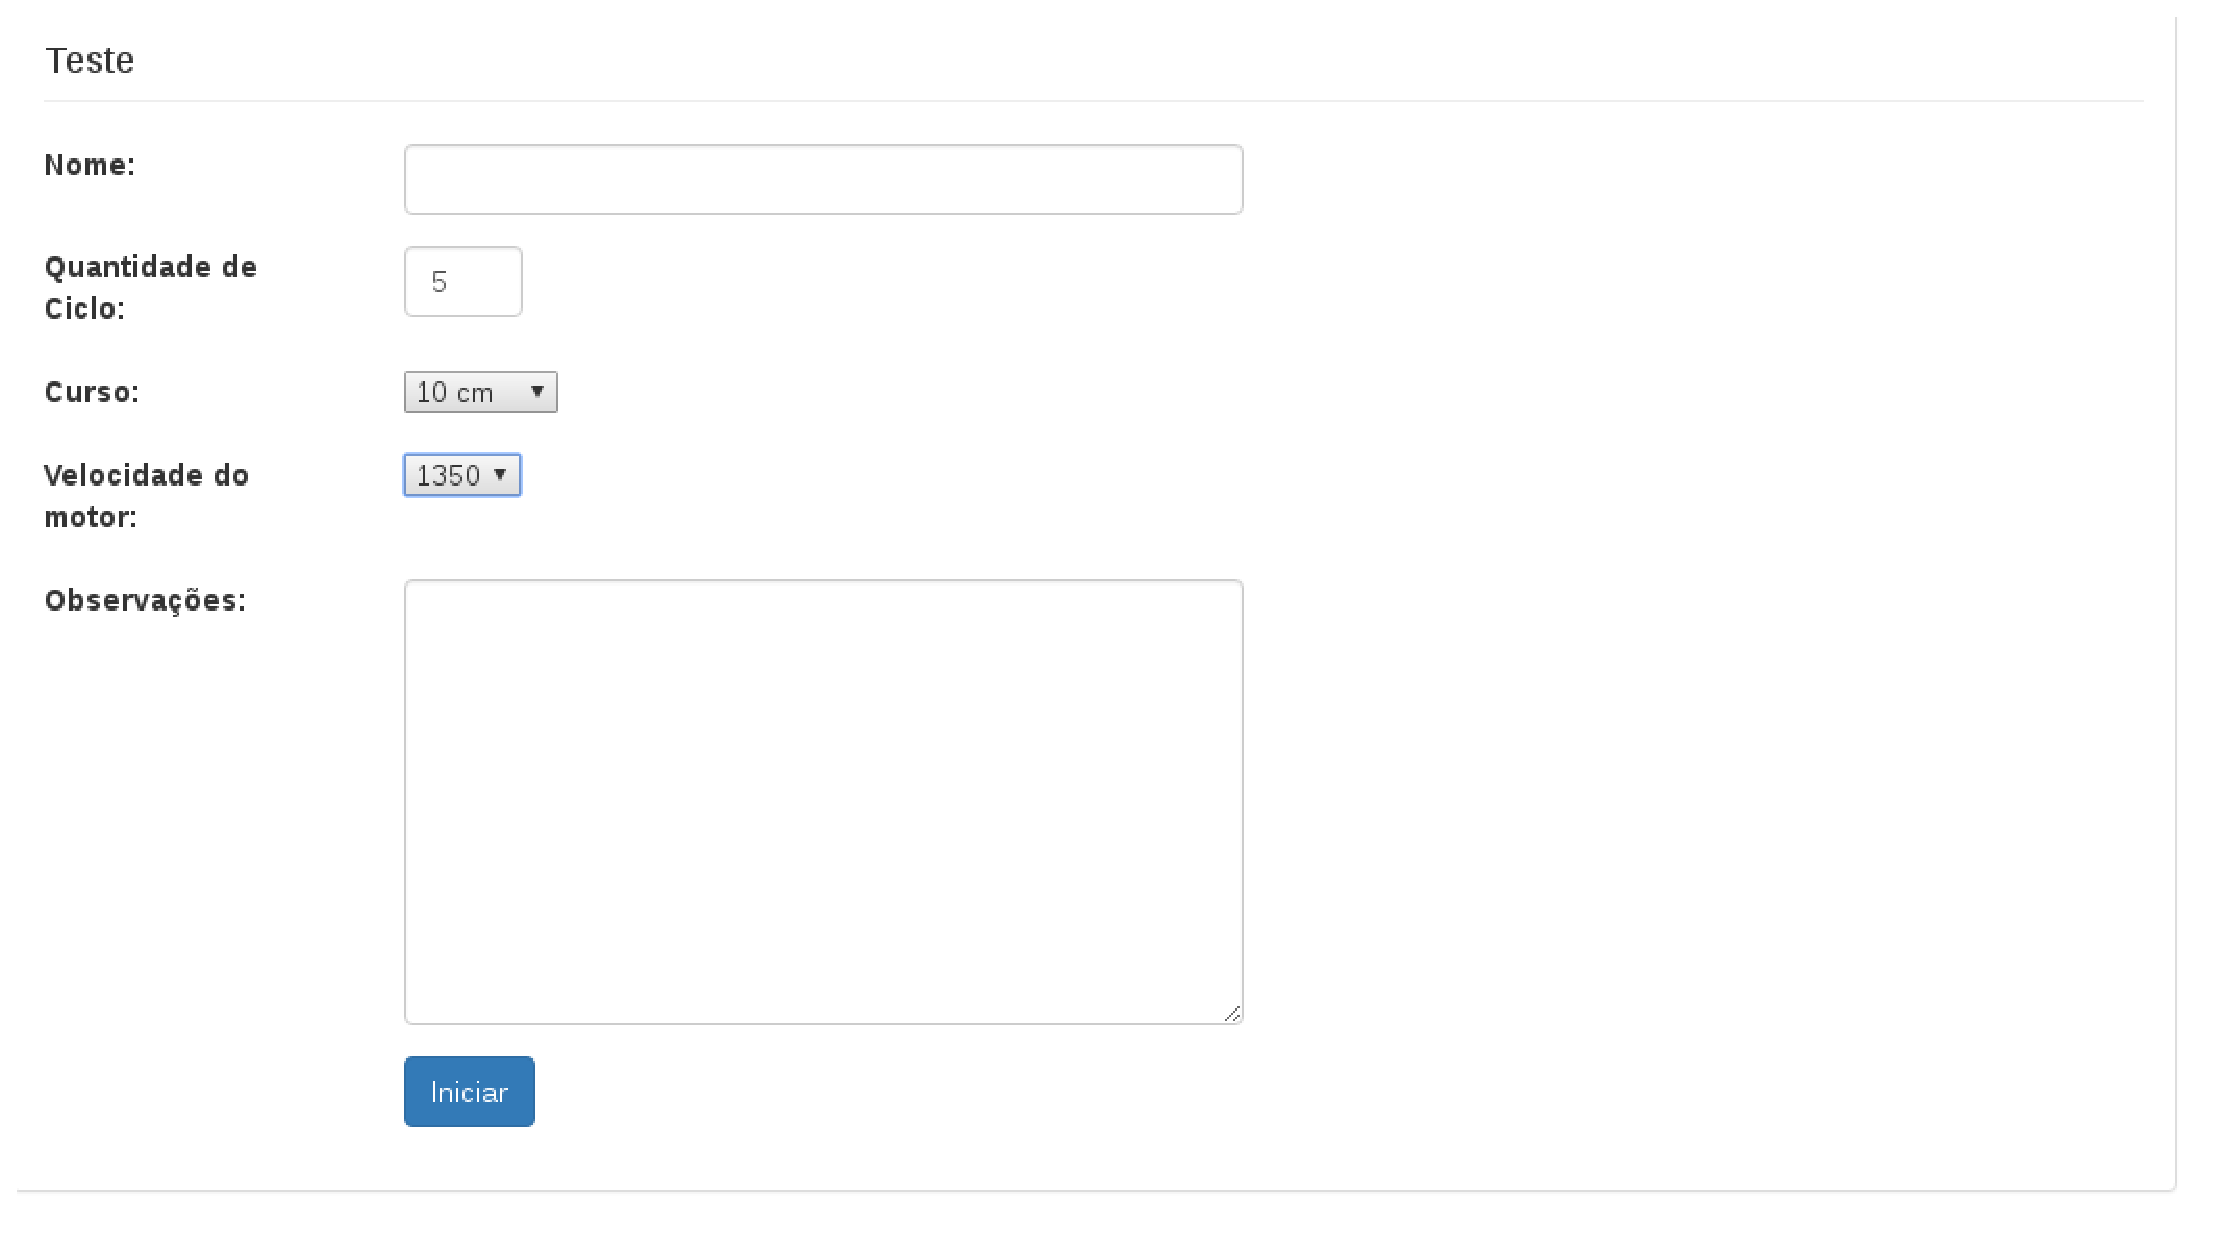
\includegraphics[width=1\textwidth]{figuras/dados_teste_fixo.eps}
	\caption{Campos do teste por velocidade fixa}
\end{figure}

O usuário irá informar o \textit{nome} do teste, a \textit{quantidade de ciclos }, o \textit{curso}, sendo que este varia entre: 10, 12.5 e 15. De acordo com o valor do \textit{curso} selecionado, o sistema irá selecionar uma velocidade. O usuário também poderá inserir \textit{observações} à respeito do teste. Quando o usuário clicar no botão \textit{iniciar} o sistema irá direcioná-lo para página de resultado do teste. 

A página de resultado do teste apresenta um cabeçalho contendo as informações básicas do teste e o gráfico de \textit{força x velocidade}. O resultado pode ser visto na Figura \ref{img:resultado}.

\begin{figure}[h]
	\centering
	\label{img:resultado}
		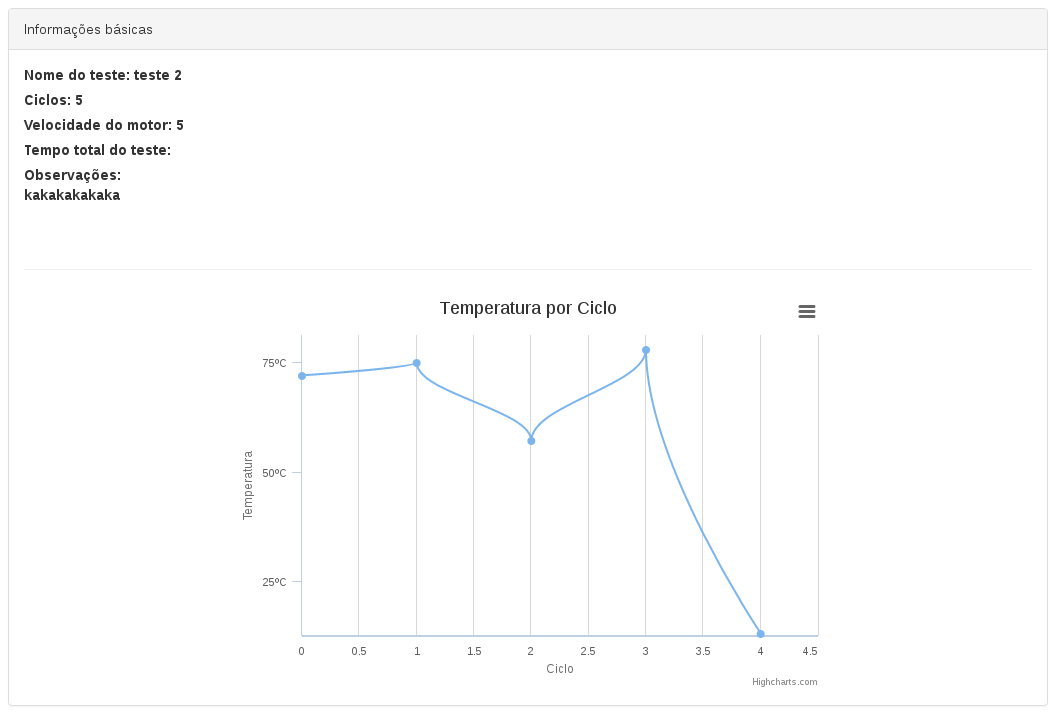
\includegraphics[width=1\textwidth]{figuras/resultado_teste_velocidade.eps}
	\caption{Resultado do teste por velocidade fixa}
\end{figure}

\section{Teste por velocidade variável}


\section{Histórico de Testes}

O histórico de teste permite que o usuário consulte os resultados de um teste já realizado. Ele está localizado no menu lateral esquerdo e pode ser acessado no link \textbf{Histórico de Testes}. Na página do histórico de teste, Figura \ref{img:historico}, o usuário consegue localizar um teste inserindo informações referentes a qualquer campo. Por exemplo, o usuário pode buscar um teste por uma data, ou ainda, algo que ele descreveu na observação. 

\begin{figure}[h]
	\centering
	\label{img:historico}
		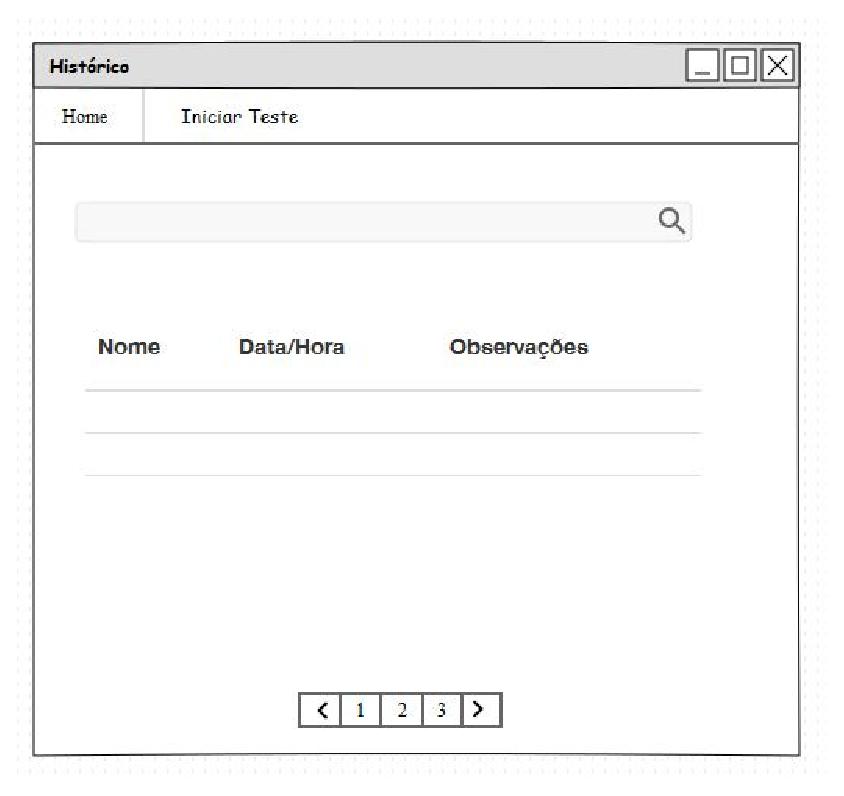
\includegraphics[width=1\textwidth]{figuras/historico.eps}
	\caption{Histórico de teste}
\end{figure}

O histórico permite realizar a filtragem da quantidade de testes que serão visualizados por página, podendo ser: 10, 25, 50 e 100.


\section{Histórico de Amortecedores}

O histórico de amortecedores pode ser acessado pelo link \textbf{Histórico de Amortecedores}, localizado no menu lateral esquerdo. Um amortecedor poderá ser localizado por código ou por valor do diâmetro externo do amortecedor.

\begin{figure}[h]
	\centering
	\label{img:historico}
		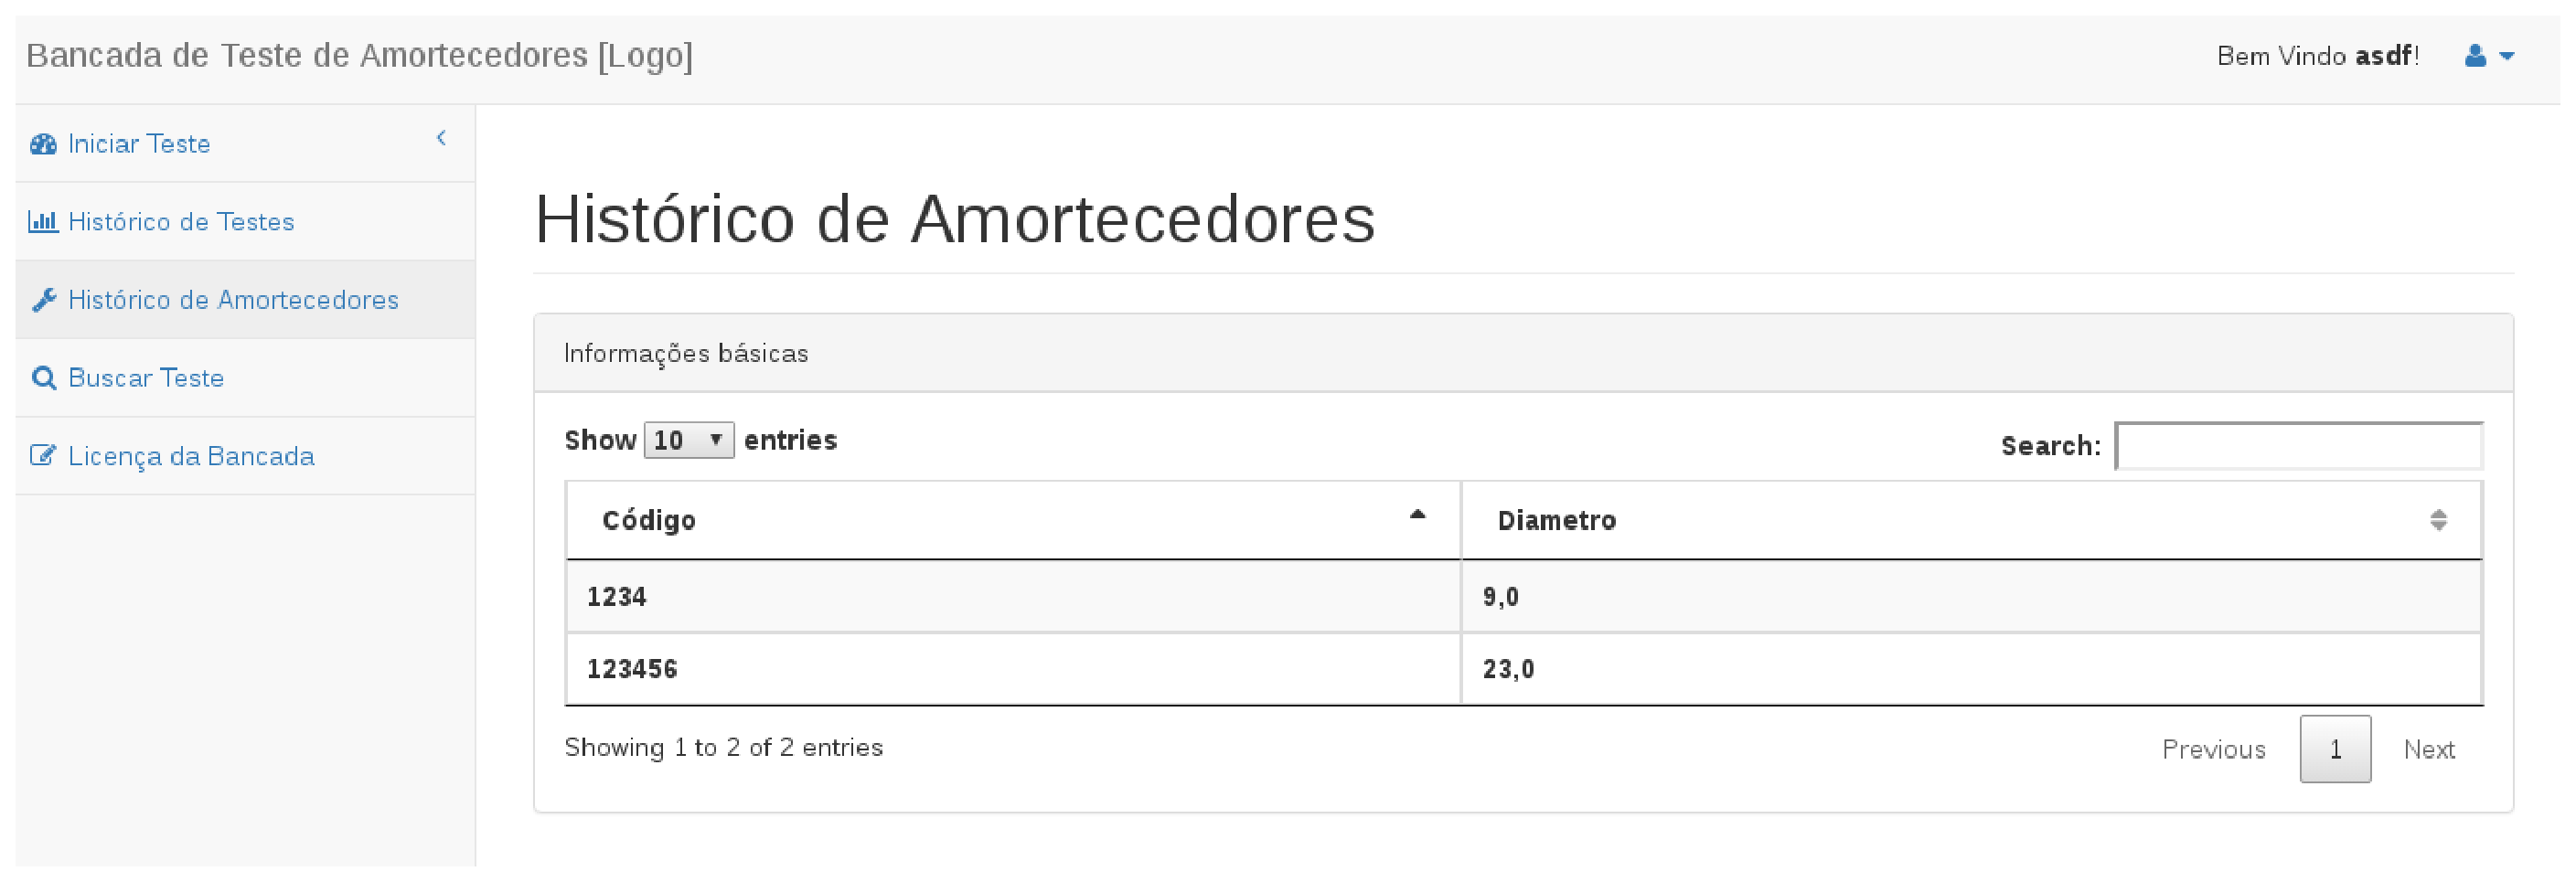
\includegraphics[width=1\textwidth]{figuras/historico_amortecedor.eps}
	\caption{Histórico de amortecedores}
\end{figure}